\chapter{Evaluation}
\label{sec:evaluation}
Im Kapitel Evaluation werden die im Kapitel 5 vorgestellten Tests evaluiert. Außerdem wird die gewählte Methode ausgewertet und
mit andere Methoden verglichen.

\section{Evaluationsmetrik}
Für das Problem von Image Colorization existiert keine relevante Evaluationsmetrik, die die Farben von den Objekten auf einem Bild auswerten kann.
Das während das Trainings angewendete Cross Entropy Loss ist nicht relevant für die Auswertung der Ergebnisse aus dem Test Datensatz. Aus diesem
Grund wurde die Evaluation der Ergebnisse durch eine Menschliche Auswertung wie bei Zhang et al. und Billaut et al.
durchgeführt.

Eine andere Evaluationsmetrik wäre ein vor-trainiertes Image Segmentation Modell. Wenn das Modell die Merkmale auf die generierten Bildern
trotzdem richtig klassifiziert, wäre davon auszugehen dass die Bilder richtig eingefärbt sind. Dieser Methode wurde nicht angewendet.

\section{Evaluation des Spiel-Datensatzes}
Mit dem Spiel-Datensatz wurde die Funktionsweise der Methode bestätigt. Die von Billaut et al. vorgeschlagene Netzwerkarchitektur für Image
colorization hat beeindruckende Ergebnisse nach wenigen Epochen erreicht. 
\\
Die gewählte Methode für das Binning funktionierte und hat ermöglicht, die originalen Farben wiederherzustellen. Die Anzahl an 
Bins war für diesen Datensatz nicht relevant da es nur 9 mögliche Farben gab.

\begin{figure}[H]
  \vspace{1cm}
  \centering
  \begin{subfigure}
    \centering
    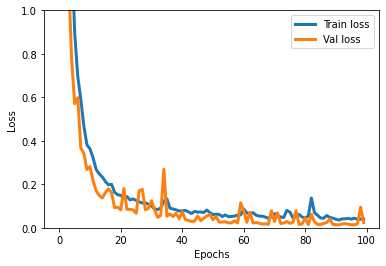
\includegraphics[width=.5\textwidth]{resources/experiments/toy_100_324_0001.png}
  \end{subfigure}
  \caption{Training und Validation Loss Verlauf des Spiel-Datensatzes}
  \label{image:toy-dataset-loss}
\end{figure}

\section{Evaluation des CIFAR-100 Subsets}
Die Ergebnissen aus dem CIFAR-100 Subset zeigten dass das Modell nach wenigen Epochen viele Merkmale lernen konnte. Ein wichtiger Faktor, der 
erwähnt werden muss, ist dass die Gewichte des Netzwerks zufällig initialisiert wurden und nicht vortrainiert waren. 
\\
\\
In diesem Datensatz wurde die Auswirkung der Bin Anzahl gemessen. Die Nutzung von 36 Bins zeigte im Vergleich zu 324 eine 
Verschlechterung der Farben in der Vorhersage. Dies ist darauf zurückzuführen dass das Modell nur 36 mögliche Farben zu Verfügung hat.
Eine Erhöhung der Bins auf 324, ermöglichte es dem Modell eine Auswahl an mehreren Farben zu treffen. 
Der Ansatz von Billaut et al. verwendet nur 32 Bins und erzielt ähnliche Ergebnisse wie die Methode dieser Arbeit mit 324 Bins.
Dies wurde erreicht in dem die Pixel von jedem Trainingsbild vor dem Training in Bins klassifiziert wurden und daraus nur die am meisten
vorkommenden 32 Bins ausgewählt wurden. Pixel die nicht in den gewählten 32 Bins klassifiziert werden konnten, wurden in das nächstliegende Bin
zugeordnet \cite{billaut2018colorunet}.
\\
\\
Die Methode mit einem MSE Loss liefert eine um ein vielfaches größere Auswahl an Farben für die Vorhersage. Bei dieser Methode treten 
die im Kapitel \ref{subsection:verwandte-arbeiten} erwähnten Schwierigkeiten auf, wobei im Falle dieses Datensatzes, die Schwierigkeiten
nur sehr latent ausgeprägt waren.
Da die Klassifikationsmethode bessere Ergebnissen geliefert hat und der Fokus der Arbeit auf Klassifikationsmethoden gesetzt war,
wurden alle Experimente des Landscape Datensatzes mit der Klassifikationsmethode durchgeführt.
\\
\\
Der Verlauf von dem Training und Validation Loss deutete bei diesem Datensatz zu \gls{overfitting}, was bei der Große des Datensatzes nicht auszuschließen war.
Wie bei \ref{section:cifar-experimente} beschrieben wurden das U-net und die Hyperparameter angepasst, um dieses zu verhindern.

\begin{figure}[H]
  \centering
  \vspace{1cm}
  \begin{subfigure}
    \centering
    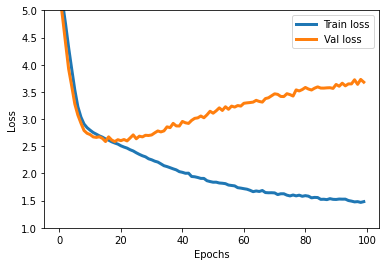
\includegraphics[width=.48\textwidth]{resources/experiments/cifar_100_324_0001.png}
  \end{subfigure}
  \begin{subfigure}
    \centering
    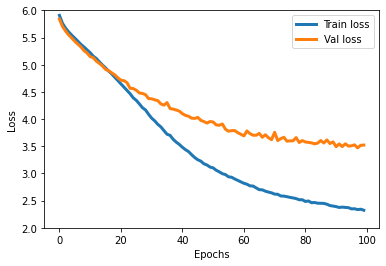
\includegraphics[width=.48\textwidth]{resources/experiments/cifar_100_324_00001.png}
  \end{subfigure}

  \caption{\gls{overfitting} auf dem CIFAR-100 Subset. \textbf{Links}: 100 Epochen mit Adam, ReLU und einer Lernrate von 0.001. \textbf{Rechts}:
  100 Epochen mit Adam, ReLU und einer Lernrate von 0.0001.}
  \label{image:gute-ergebnisse-cifar}
\end{figure}

Eine Anpassung der Lernrate führte nur zu einem langsameren Training. Eine Reduktion der lernbaren Parameter von 135684 auf 35748 zeigte 
eine deutliche Verbesserung der Performance des Modells und reduzierte das \gls{overfitting}.

\begin{figure}[H]
  \centering
  \vspace{1cm}
  \begin{subfigure}
    \centering
    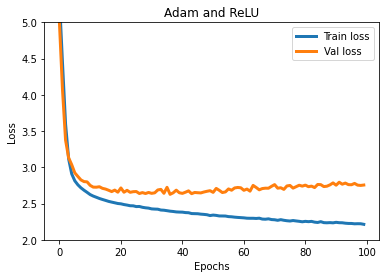
\includegraphics[width=.48\textwidth]{resources/experiments/cifar-adam-relu.png}
  \end{subfigure}
  \begin{subfigure}
    \centering
    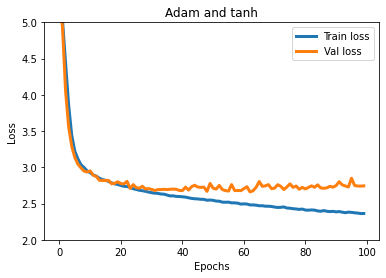
\includegraphics[width=.48\textwidth]{resources/experiments/cifar-adam-tanh-100.png}
  \end{subfigure}

  \caption{Loss Verlauf mit einer reduzierten Anzahl an Parametern und verschiedenen Aktivierungsfunktionen. 
  \textbf{Links}: 100 Epochen mit Adam, ReLU und einer Lernrate von 0.001. \textbf{Rechts}: 100 Epochen mit Adam, Tanh und einer Lernrate von 0.001.}
  \label{image:gute-ergebnisse-cifar}
\end{figure}

Der Grund für das \gls{overfitting} ist in diesem Fall auf die Große des Subsets zurückzuführen. Um das zu prüfen wurde das Modell auf dem kompletten CIFAR-100
Datensatz für 150 Epochen trainiert, was einen guten Loss Verlauf zeigte. Andererseits, hat das Modell nichts relevantes gelernt und 
konnte kein Bild richtig einfärben, was bei der Anzahl der Klassen und der Anzahl der Epochen nichts ungewöhnliches ist.

\section{Evaluation des Landscape Datensatzes}
Die Ergebnisse dieses Modells zeigen, dass die ausgewählte Methode mit wenigen Bildexemplaren und Epochen, sehr gute Ergebnisse erreichen kann.
Die Anzahl der Bins für diesen Datensatz wurde durch die Ergebnisse der vorgeführten Experimenten auf 324 gesetzt, da diese Anzahl die beste Kombination
aus Trainingszeit und Performance gezeigt hat.
\\
\\
Der Loss Verlauf der Experimente deutete bei diesem Datensatz ebenfalls nach wenige Epochen auf \gls{overfitting} hin. Nach Zahlreichen Experimenten
konnte das \gls{overfitting} durch Anpassung der Hyperparameter nur minimiert werden. Für die Auswertung der Ergebnisse wurde das Modell mit dem besten
Validation Loss verwendet.
\\
\\
Bei der Evaluation der Ergebnisse ist zu erkennen, dass schon nach den wenigen Epochen das Modell in der Lage ist die wichtigsten Entitäten wie den Himmel, Wolken, Wasser,
Grass und Erde richtig einzufärben. Es fällt auf, dass bei einigen Bildern die Vorhersage des Modells realer aussieht, als das Original Bild,
wie im zweiten Beispiel von \ref{image:gute-ergebnisse-own} zu sehen ist. Im Vergleich zum Modell von Billaut et al. sehen die vorhergesagten 
Farben von diesem Modell sehr ähnlich aus. Das zeigt, dass die Performance der Methode ohne die Optimierungstechniken vergleichbar ist.
Die Auswirkung des Temperaturwerts ist bei beiden Modellen ähnlich. Der Modus der Verteilung zeigt einen rötlichen Ton bei den
Ergebnissen und der Durchschnitt zeigt bei einigen Fällen gesättigte Bilder.
\\
Da die Datensatz Größe von Billaut et al. fast identisch zu der Datensatz Größe dieser Arbeit ist, könnte das Problem mit dem \gls{overfitting}
auf die Qualität des Datensatzes zurückzuführen sein. Der Loss Verlauf zeigt kein \gls{overfitting} und das verwendete U-Net ist ähnlich zum
U-Net der vorliegenden Arbeit, was ein \gls{overfitting} wegen der angewendeten Netzwerkarchitektur ausschließt. 
\\
\\
Ein Vergleich mit den Ergebnissen von Zhang et al. wäre nur angemessen mit den Ergebnissen aus deren Klassifikationsmodell ohne Rebalancing.
In diesem Fall sind die Resultate dieses Models nicht weit entfernt von deren Ergebnissen. Es ist zu erkennen, dass deren Ergebnisse ähnliche
Merkmale mit den Ergebnissen dieser Arbeit vorweisen, wie z.B. die Ähnlichkeit der Vorhersagen zwischen Klassifikationsmethode und Regressionsmethode.
Die Ergebnissen mit Class Rebalancing unterscheiden sich deutlicher von den Ergebnissen der Regressionsmethode. 
Da deren Datensatz über 1.5 Millionen Bilder beinhaltet, kann das Modell mehr Objekte auf den
Bildern einfärben, was sich bei einigen Bildern z.B. mit Menschen, bemerkbar macht. 
\\
\\
Im allgemeinen sind die Ergebnisse dieses Modells mit anderen Ergebnissen von Klassifikationsmethoden ohne Optimierungstechniken wie Class Rebalancing
vergleichbar.